\chapter{Background} \label{ch:background}

This chapter introduces the biological and neuromorphic ideas used in the model. The aim is not to reproduce bat auditory biology in full anatomical detail. Instead, the background is organised around the key computations needed for active acoustic localisation: 
\begin{enumerate}
    \item extracting timing, level, and spectral cues from an echo,
    \item representing those cues as neural population codes,
    \item decoding those populations into distance, azimuth, and elevation estimates.
\end{enumerate}
These ideas are discussed in relation to the model developed in this project, while recognising that the biological anatomy and systems are substantially more complex.


\section{Echolocation as Active Localisation}

Echolocating bats localise objects by emitting an acoustic call and analysing the returning echo. This is an active sensing problem rather than passive listening. The animal knows approximately what signal it emitted, when it emitted it, and how that signal should change after reflection from a target. The returning echo, therefore, carries cues for distance, azimuth, and elevation. These cues are not independent, as the same echo amplitude, frequency content, and arrival time are affected by target range, head geometry, ear shape, and environmental noise. The biological problem is to separate these interacting effects quickly enough to guide flight.

\begin{figure}[h]
    \centering
    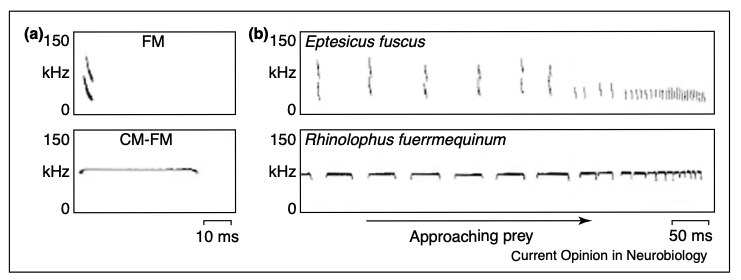
\includegraphics[width=0.86\linewidth]{2_Background/background_figures/Auditory_localisation/bat_call.png}
    \caption{Echolocation signal structures. (a) Examples of FM and CF components used by echolocating bats. (b) Signal sequences produced while pursuing prey; pulse rate increases and call duration decreases as the bat approaches the target \cite{MossANeurobiologyBats}.}
    \label{fig:bat_call_redraft}
\end{figure}

Bats are a useful inspiration because their sensing problem is similar to a radar problem, but is solved by a compact, event-driven nervous system. Many echolocating species use frequency-modulated (FM) sweeps, sometimes with constant-frequency (CF) components, as shown in Figure~\ref{fig:bat_call_redraft}. A delayed echo can be matched against an internal copy (or efference copy) of the emitted signal, while the echo spectrum can also carry elevation information. The bat is essentially listening out for its own call and measuring the changes that the call has undergone. 



Species using CF--FM signals typically forage in dense foliage, using Doppler shifts and an acoustic fovea in the auditory cortex to estimate relative velocity and improve target tracking \cite{MossANeurobiologyBats,Ulanovsky2008WhatBrain}. By contrast, many FM bats forage in the open, using shorter-duration broadband signals that are well suited to three-dimensional (3D) target localisation \cite{MossANeurobiologyBats}. This project therefore uses an FM sweep because the target variable is 3D position rather than velocity. The model uses a single pulse emission to simplify the problem to static object localisation.

\section{Auditory Cues for 3D Position}

Many auditory cues contain information about an object's position in 3D space. We will discuss the main ones that are primarily used.

\subsection{Distance}

In passive listening, absolute range is difficult because the original source intensity is unknown. Active echolocation provides a stronger cue: time-of-flight (ToF). If an emitted call reflects from a target and returns after delay $\Delta t$, the target range is approximately
\begin{equation}
    r = \frac{v_{sound} \cdot \Delta t}{2},
    \label{eq:tof_distance_redraft}
\end{equation}
where $v_{sound}$ is the speed of sound and the factor of two accounts for the outward and return path. This is the main distance cue used in the model of this project. Echo amplitude also decreases with propagation distance, but intensity is less reliable because it depends on target reflectivity, call intensity, ear direction, and environmental conditions.

The biological complication is that the brain does not contain a simple digital clock. It must represent delay using neural signals. In bats, delay-sensitive neurons respond selectively to particular pulse-echo ToF delays, so range can be represented as activity over a bank of candidate delays rather than as a single stopwatch value \cite{Suzuki2017AcuityBats}.

\subsection{Azimuth}

\begin{figure}[h]
    \centering
    \begin{subfigure}[t]{0.5\textwidth}
        \textbf{\large A}\\[0.5ex]
        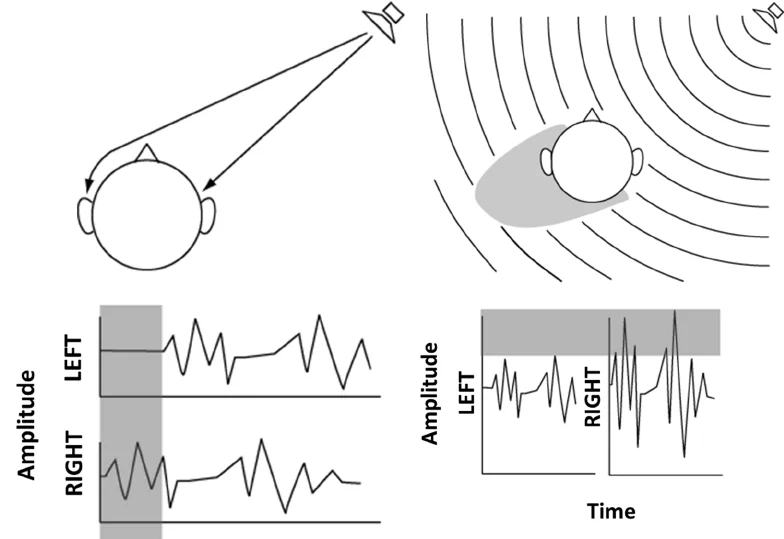
\includegraphics[height=4.8cm]{2_Background/background_figures/Auditory_localisation/itd_ild.png}
        \caption{}
    \end{subfigure}
    \hspace{0.1cm}
    \begin{subfigure}[t]{0.32\textwidth}
        \textbf{\large B}\\[0.5ex]
        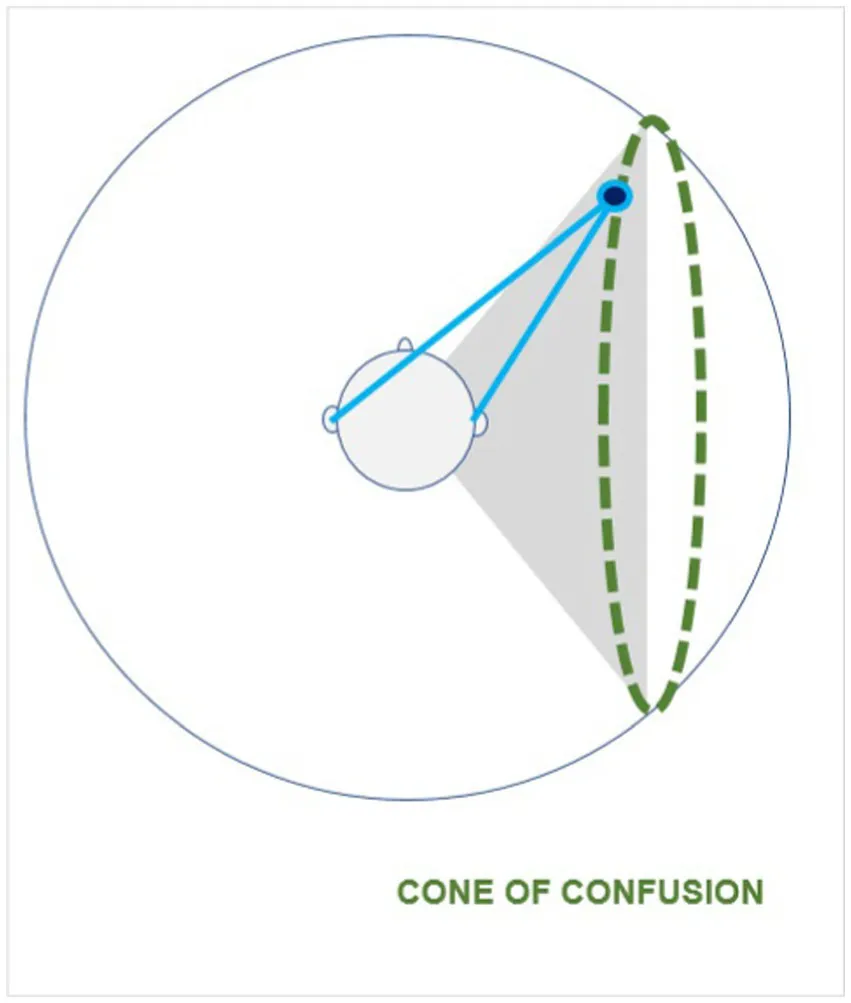
\includegraphics[height=4.8cm]{2_Background/background_figures/Auditory_localisation/cone.png}
        \caption{}
    \end{subfigure}
    \caption{A: ITD and ILD cues. B: cone of confusion for constant ITD \cite{Sun2015DynamicListeners,Carlini2024AuditoryReview}.}
    \label{fig:azimuth_cues_redraft}
\end{figure}

Azimuth is the horizontal angle of the target. It is mainly estimated using binaural differences: the difference between the signals at the two ears. The first cue is interaural time difference (ITD), the arrival-time difference between ears. In a simple straight-line approximation,
\begin{equation}
    \theta = \arcsin\left(\frac{v_{sound}\cdot\mathrm{ITD}}{d}\right),
    \label{eq:itd_azimuth_redraft}
\end{equation}
where $\theta$ is azimuth and $d$ is the interaural distance. This ignores diffraction around the head, but it captures the key computational idea: a timing difference maps monotonically to horizontal angle over the frontal region.

The second cue is interaural level difference (ILD), the amplitude difference between the two ears. At high frequencies the head casts an acoustic shadow, reducing sound level at the far ear. Because bat calls are high frequency, ILD can be a strong azimuth cue, although its reliability depends on head size, frequency, and source direction. The classical duplex theory states that ITD is most useful at low frequencies and ILD at high frequencies \cite{Rayleigh1907Direction}. For this project, the important point is simpler: timing and level comparisons provide complementary azimuth evidence.

ITD alone is ambiguous. A cone of directions can share the same interaural delay, as shown in Figure~\ref{fig:azimuth_cues_redraft}. This is one reason why elevation-dependent spectral cues and multiple cue pathways are needed.



\subsection{Elevation}

Elevation is the vertical angle of the target. Because the left and right ears are mostly separated horizontally, binaural timing and level differences are weaker vertical cues. Instead, elevation is strongly linked to spectral filtering by the outer ear, or pinna. A sound arriving from different vertical angles reflects from the ridges of the pinna in different ways, producing direction-dependent peaks and notches in the spectrum. The full direction-dependent filtering of the head, torso, and outer ears is called the head-related transfer function (HRTF) \cite{Carlini2024AuditoryReview,Zonooz2019SpectralElevation}.

The simplified model in this project therefore needs an elevation cue that preserves the same physical problem: elevation must be inferred from a frequency-dependent spectral shape rather than from a simple time delay. A comb filter is used because it produces a moving pattern of spectral notches in a physically motivated way, approximating the interference caused by delayed pinna reflections. This is more representative than imposing an arbitrary notch using a Butterworth band-stop or band-pass filter, although it remains much simpler than a measured HRTF. The implementation is described in Chapter~\ref{ch:modelling}. Figure~\ref{fig:elevation_cues_redraft} shows the biological pinna mechanism and the kind of elevation-dependent HRTF map that motivates this abstraction.

\begin{figure}[H]
    \centering
    \begin{subfigure}[t]{0.45\textwidth}
        \textbf{\large A}\\[0.5ex]
        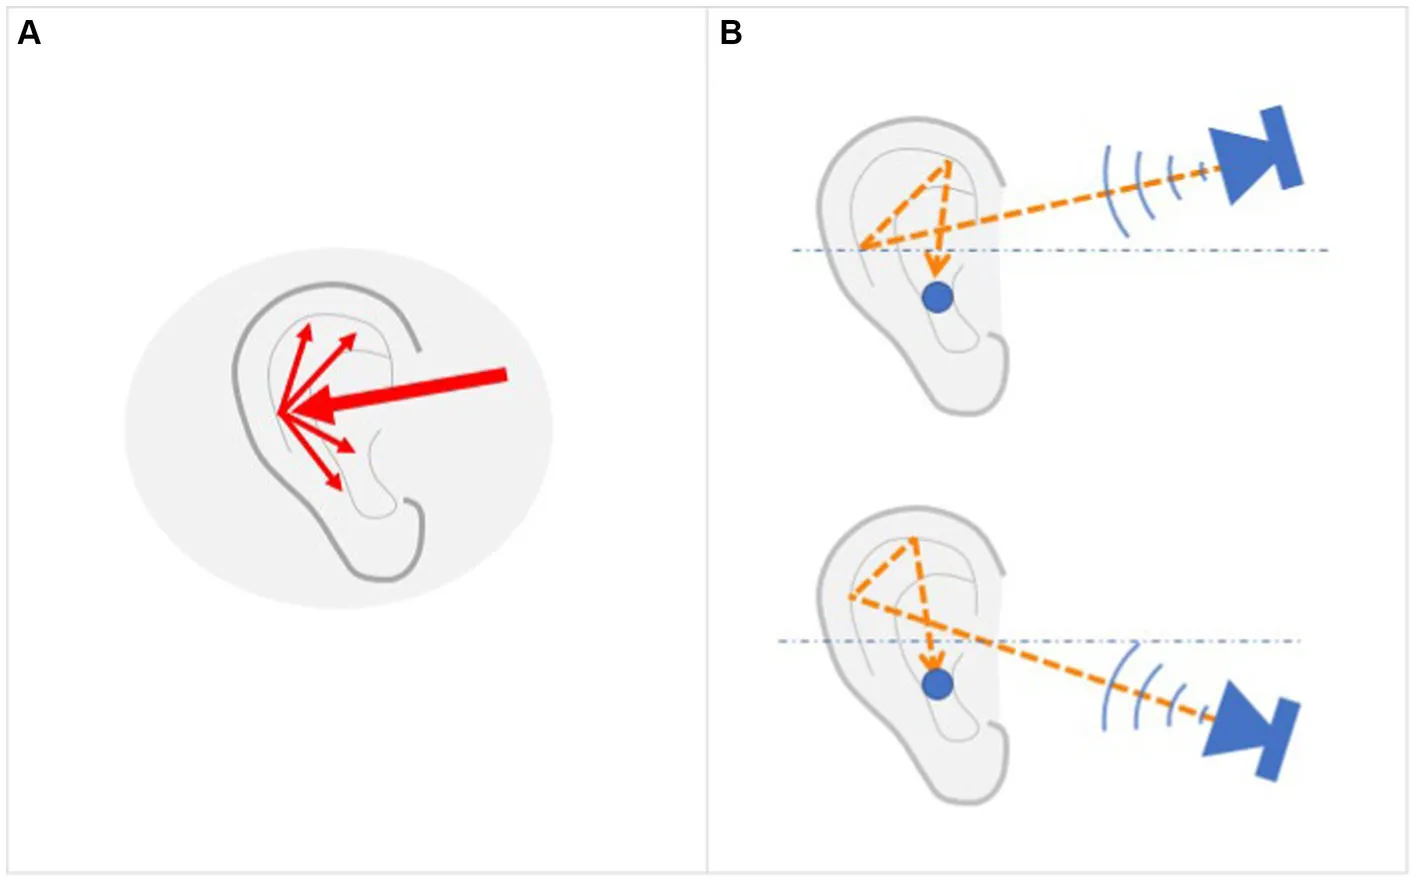
\includegraphics[height=3.8cm]{2_Background/background_figures/Auditory_localisation/pinna_1.png}
        \caption{}
    \end{subfigure}
    \hspace{0.1cm}
    \begin{subfigure}[t]{0.45\textwidth}
        \textbf{\large B}\\[0.5ex]
        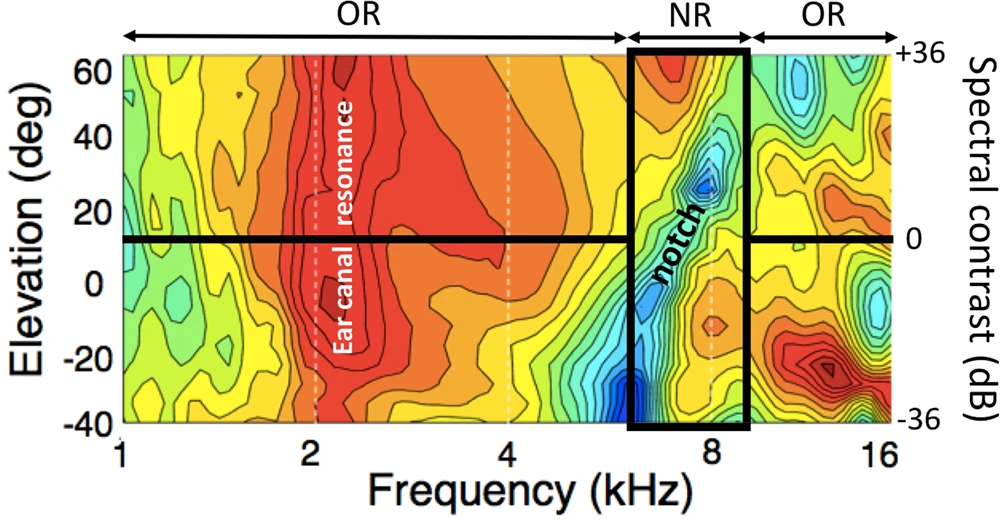
\includegraphics[height=3.8cm]{2_Background/background_figures/Auditory_localisation/pinna_map.png}
        \caption{}
    \end{subfigure}
    \caption{A: pinna-based HRTF mechanism. B: measured elevation-dependent HRTF structure, with red indicating high gain and blue indicating low gain \cite{Carlini2024AuditoryReview,Zonooz2019SpectralElevation}.}
    \label{fig:elevation_cues_redraft}
\end{figure}

\section{Biological Auditory Pathways as Computation}
\label{sec:biology}

The bat auditory system is highly specialised, but the model in this report uses a functional abstraction rather than a full anatomical simulation. Figure~\ref{fig:overall_pathway_redraft} shows the key biological scaffold. The left side shows the ascending auditory pathway, where acoustic signals are transformed into neural representations. The right side shows descending and vocalisation pathways, which are simplified into an emitted call and a corollary discharge in the model. A corollary discharge is an internal copy of a self-generated motor command or expected sensory signal. In echolocation, it provides a reference against which the returning echo can be compared.

\begin{figure}[H]
    \centering
    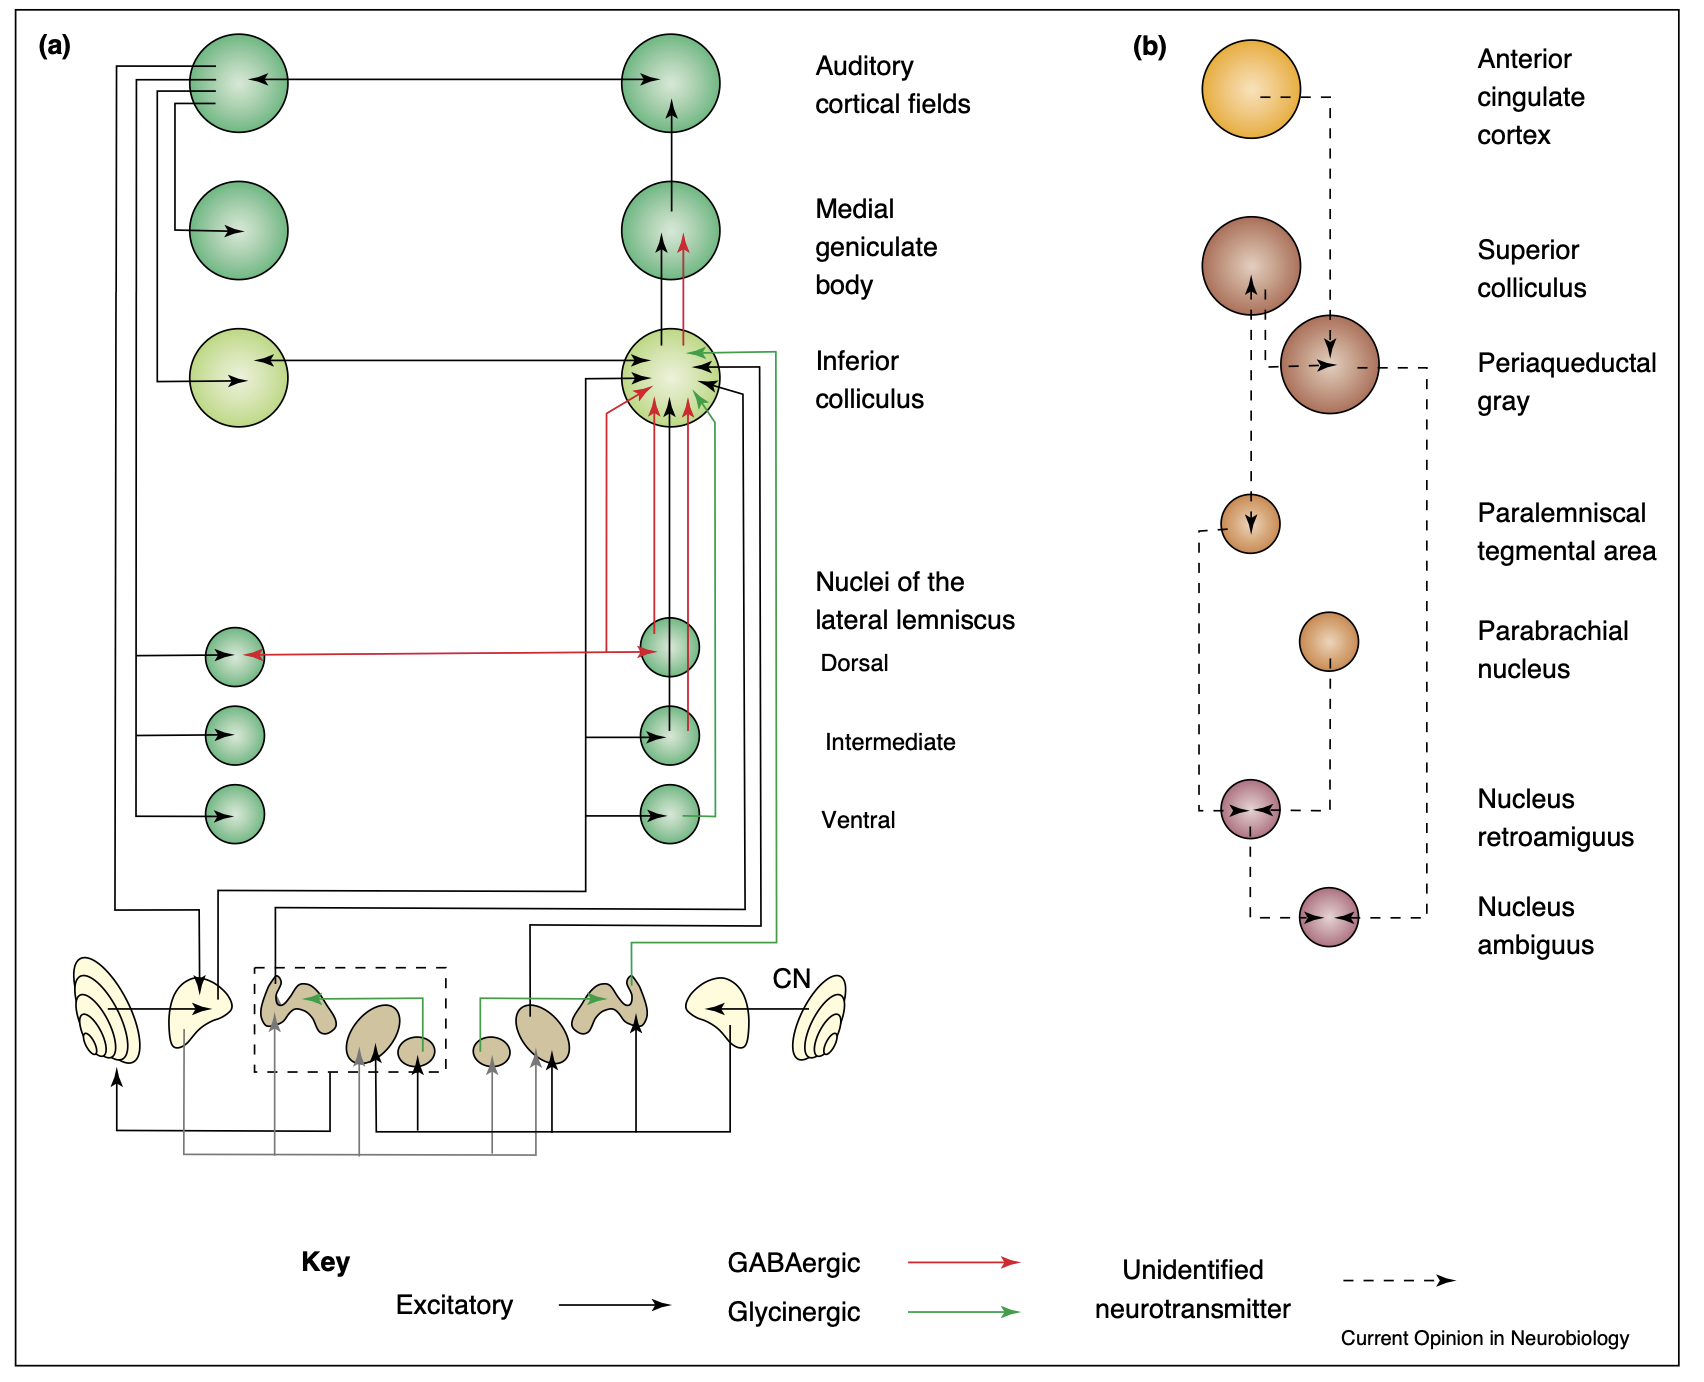
\includegraphics[width=\textwidth]{2_Background/background_figures/biology/overall_brain.png}
    \caption{Major ascending auditory connections and descending vocalisation circuitry in bat echolocation \cite{MossANeurobiologyBats}. In this project the detailed vocalisation pathway is simplified to an emitted call and a corollary-discharge copy, while the ascending pathway motivates the cochlea, distance, azimuth, elevation, and SC readout modules. The dashed box contains the superior olivary complex, comprising the MSO, LSO, and MNTB brain areas.}
    \label{fig:overall_pathway_redraft}
\end{figure}

The modelling principle is that each biological region is treated as a computing block. The aim is to identify the localisation cue processed by a region and the form of neural representation passed downstream. The spiking abstractions used to implement these computations are introduced in the following section.

\subsection{Cochlea and Tonotopic Encoding}

The cochlea converts air-pressure waveforms into neural activity. It is tonotopic, meaning different positions along the cochlea respond preferentially to different frequencies. High frequencies peak near the base, lower frequencies further along the basilar membrane. This spatial frequency decomposition is shown in Figure~\ref{fig:cochlea_redraft}. The output is not a continuous spectrogram but a set of neural signals from frequency-selective channels.

\begin{figure}[H]
    \centering
    \begin{subfigure}[t]{0.45\textwidth}
        \textbf{\large A}\\[0.5ex]
        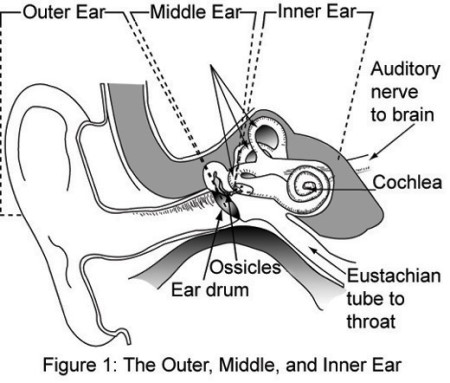
\includegraphics[height=3.8cm]{2_Background/background_figures/biology/cochlea.png}
        \caption{}
    \end{subfigure}
    \hspace{0.1em}
    \begin{subfigure}[t]{0.45\textwidth}
        \textbf{\large B}\\[0.5ex]
        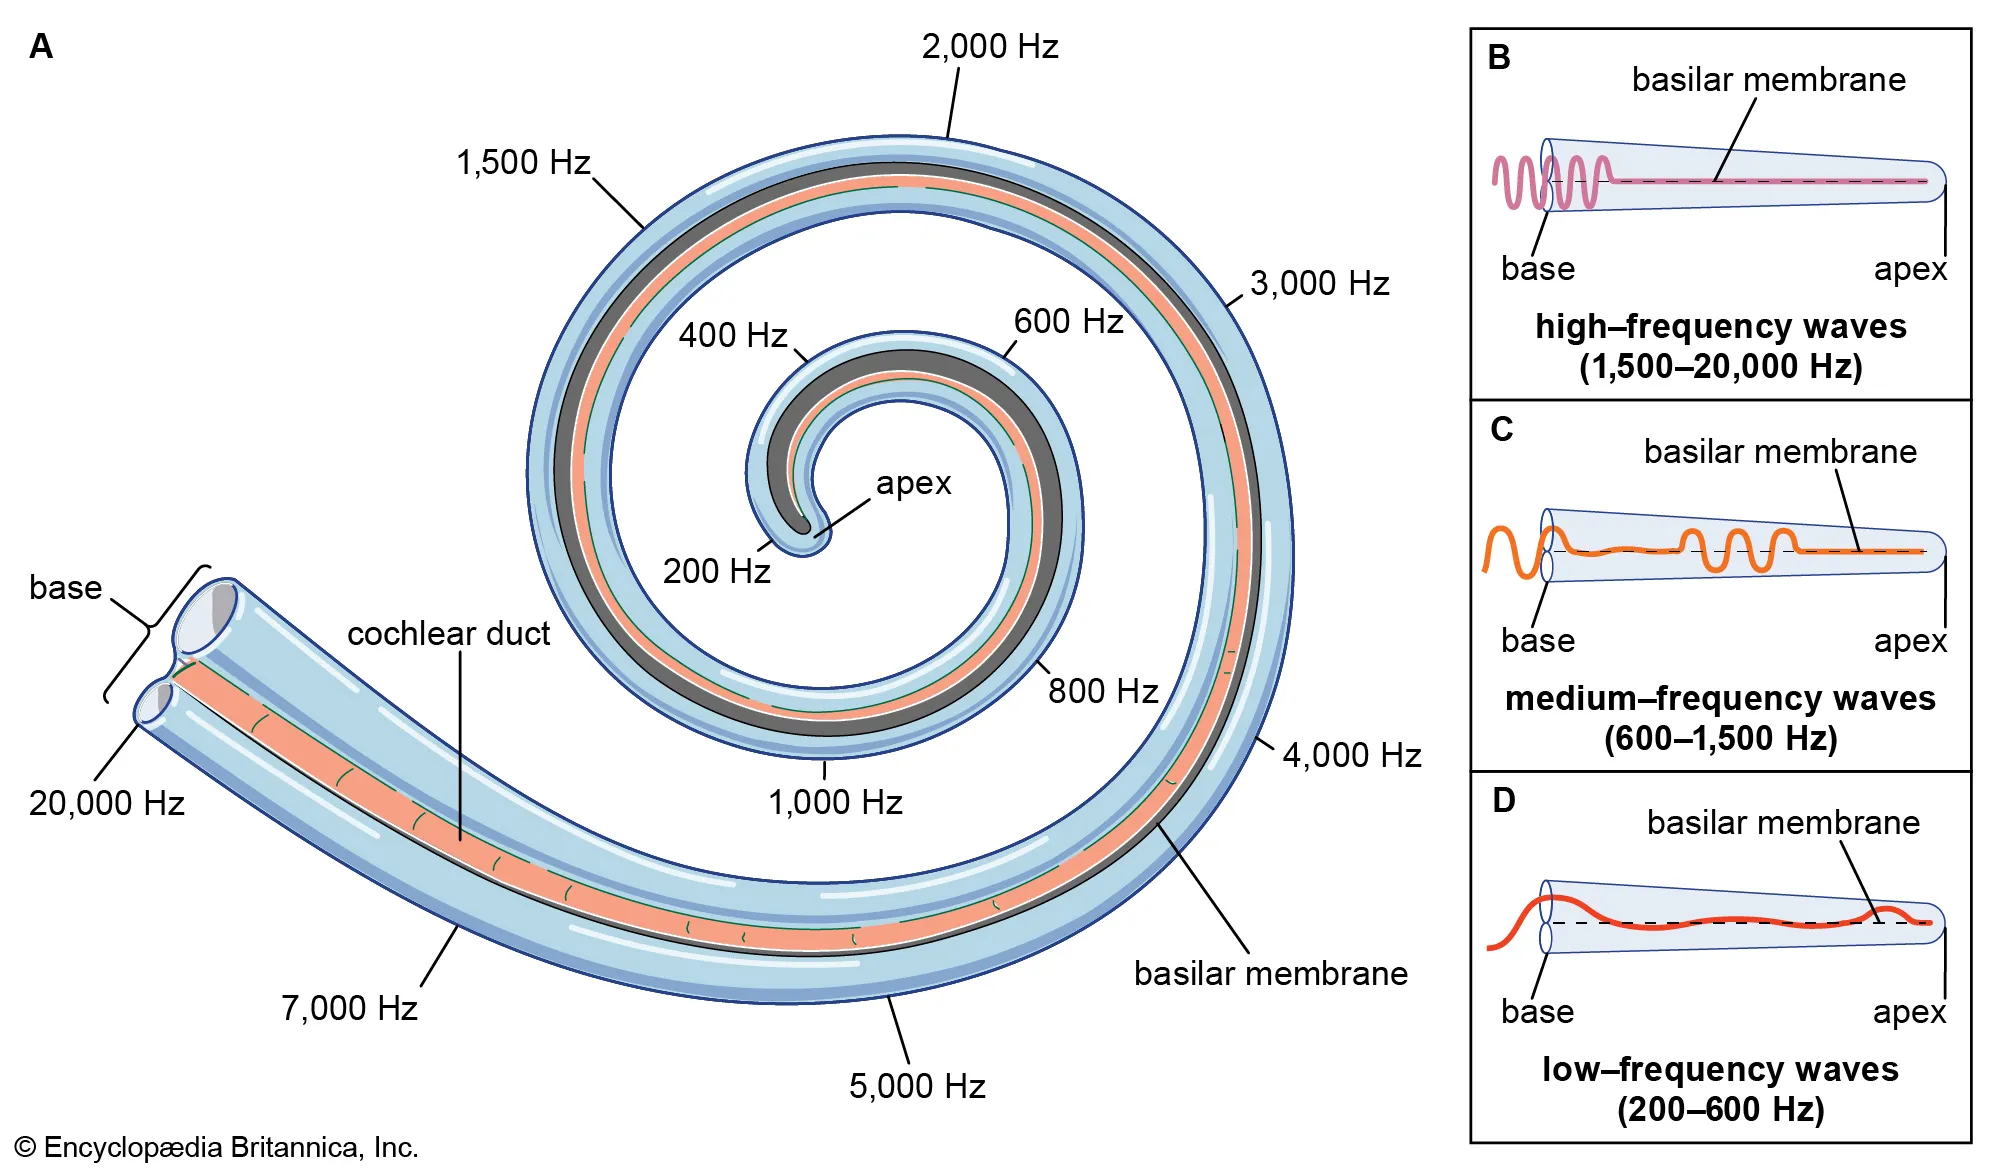
\includegraphics[height=3.8cm]{2_Background/background_figures/biology/spiral.png}
        \caption{}
    \end{subfigure}
    \caption{A: outer, middle, and inner ear. B: tonotopic frequency organisation along the cochlea \cite{CochleaStudy.com,HumanBritannica}.}
    \label{fig:cochlea_redraft}
\end{figure}

In the model, this motivates a cochlear filterbank followed by spike encoding. The exact biophysics of basilar-membrane fluid mechanics are not simulated. Instead, the cochlea is abstracted as a bank of frequency-selective filters whose outputs are converted into cochlear spike rasters. This retains the computational features needed later: frequency selectivity, timing, and sparse events.

\subsection{Cochlear Nuclei and Pathway Splitting}

After the cochlea, auditory nerve fibres project to the cochlear nuclei (CN). The CN can be understood as an early router and feature extractor. Ventral cochlear nucleus (VCN) neurons are specialised for preserving precise timing and onset information. This matters for distance and ITD, where sub-millisecond timing errors can shift the inferred position. The dorsal cochlear nucleus (DCN) is more closely associated with spectral processing and is therefore relevant to elevation cues.

The biological details are richer than this abstraction, but the functional split is the important part for the report. The model uses VCN/VNLL-inspired onset processing to clean the cochlear spike raster before distance and azimuth coincidence detection. For elevation, the model uses a DCN-like spectral population that compares the observed frequency profile with expected comb-filter templates.

\subsection{Superior Olivary Complex and Binaural Comparison}

The superior olivary complex (SOC) provides an early stage of binaural comparison. The medial superior olive (MSO) is associated with sensitivity to interaural time differences: timing-sensitive inputs from the two ears are compared, motivating the Jeffress-style coincidence population used later in the report. The lateral superior olive (LSO) supports interaural level-difference processing. LSO neurons receive excitation driven by the ipsilateral (same-side) ear and inhibition driven by the contralateral (opposite-side) ear through the medial nucleus of the trapezoid body (MNTB). The balance between these inputs produces a rate code for binaural level difference. These pathways are shown in Figure \ref{fig:SOC}.

\begin{figure}[h]
    \centering
    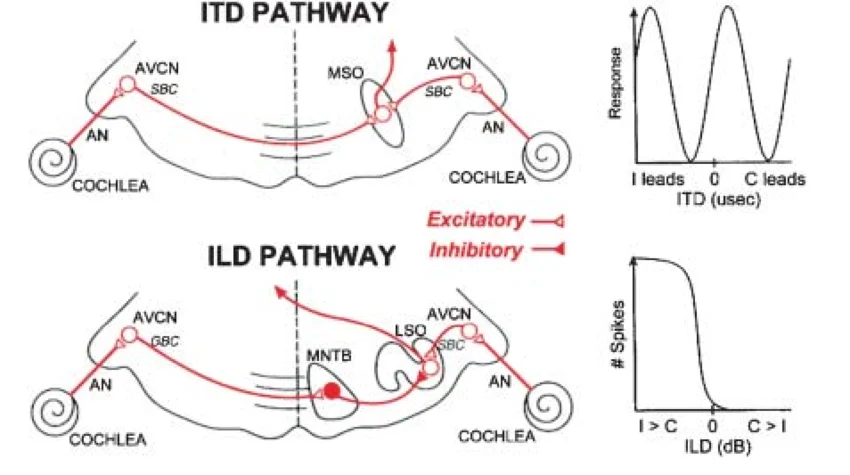
\includegraphics[width=0.6\textwidth]{2_Background/background_figures/biology/SOC.png}
    \caption{ITD and ILD pathways in the brain of a mammal \cite{Tollin2003TheLocalization}.}
    \label{fig:SOC}
\end{figure}

The relative importance of ITD and ILD depends on species, frequency, and acoustic context. The model therefore retains both cues: an MSO-style timing population and an LSO/MNTB-style opponent population. These are functional abstractions of binaural comparison rather than detailed simulations of the underlying circuitry.

\subsection{Nuclei of the Lateral Lemniscus}

The nuclei of the lateral lemniscus (NLL) provide an intermediate stage between the cochlear nuclei and the inferior colliculus. In echolocating bats, neurons in the ventral nucleus of the lateral lemniscus (VNLL) can respond precisely to sound onset, providing temporal markers for later processing. The dorsal nucleus of the lateral lemniscus (DNLL) is an inhibitory nucleus that contributes to shaping timing-sensitive responses in the inferior colliculus. In this project, these roles motivate two simplified operations: a combined VCN/VNLL-style onset preservation and DNLL-style suppression of late activity. The implemented suppression stage is a functional abstraction for single-target localisation rather than a detailed model of DNLL circuitry.

\subsection{Midbrain and Cortical Population Maps}

The inferior colliculus (IC) and auditory cortex (AC) contain neurons sensitive to combinations of timing, frequency, and binaural cues. For distance, FM-FM delay-tuned neurons (neurons with varying time delays that respond to certain frequencies) respond strongly when an emitted-call component and an echo component arrive with a particular delay \cite{Suga2015NeuralBat,Suzuki2017AcuityBats}. For azimuth, binaural timing and level differences are compared across neural populations. For elevation, spectral shape can be mapped into a population of candidate elevations.

The key modelling choice is therefore to represent each coordinate as a population code. A population code stores a value as a pattern of activity across many neurons, each tuned to a candidate coordinate. A single neuron might represent ``about 3 ms delay'' or ``about +20 degrees elevation'', but the final estimate can be decoded from the whole activity pattern. The importance of this distributed readout is developed after the spiking computation section.

\subsection{The SC as a Readout Abstraction}

The superior colliculus (SC) is involved in spatial orienting and sensorimotor maps. In this project it is treated as the final coordinate-readout stage rather than as a detailed motor-control model. The remaining descending vocalisation pathway is collapsed into two model components: the emitted call and the corollary-discharge copy used by the distance pathway. This is a deliberate simplification. It keeps the model focused on localisation while preserving the core active-sensing idea: the brain compares an internally available reference with the returning echo.

\section{Spiking Computation}

Spiking neural networks (SNNs) use event-like spikes rather than continuously valued activations. These spikes can be thought of as Kronecker delta functions. Neuron models are used effectively as kernels or activation functions for these spikes. A standard leaky integrate-and-fire (LIF) neuron model provides a useful abstraction between biophysical detail and an artificial neural-network unit. It integrates input current into a membrane voltage, the membrane leaks over time, and the neuron emits a spike when its voltage crosses a threshold. The passive membrane can be interpreted as an RC circuit, as shown in Figure~\ref{fig:lif_circuit}. 

\begin{figure}[H]
    \centering
    \begin{minipage}[b]{0.40\textwidth}
        \vspace{0pt}
        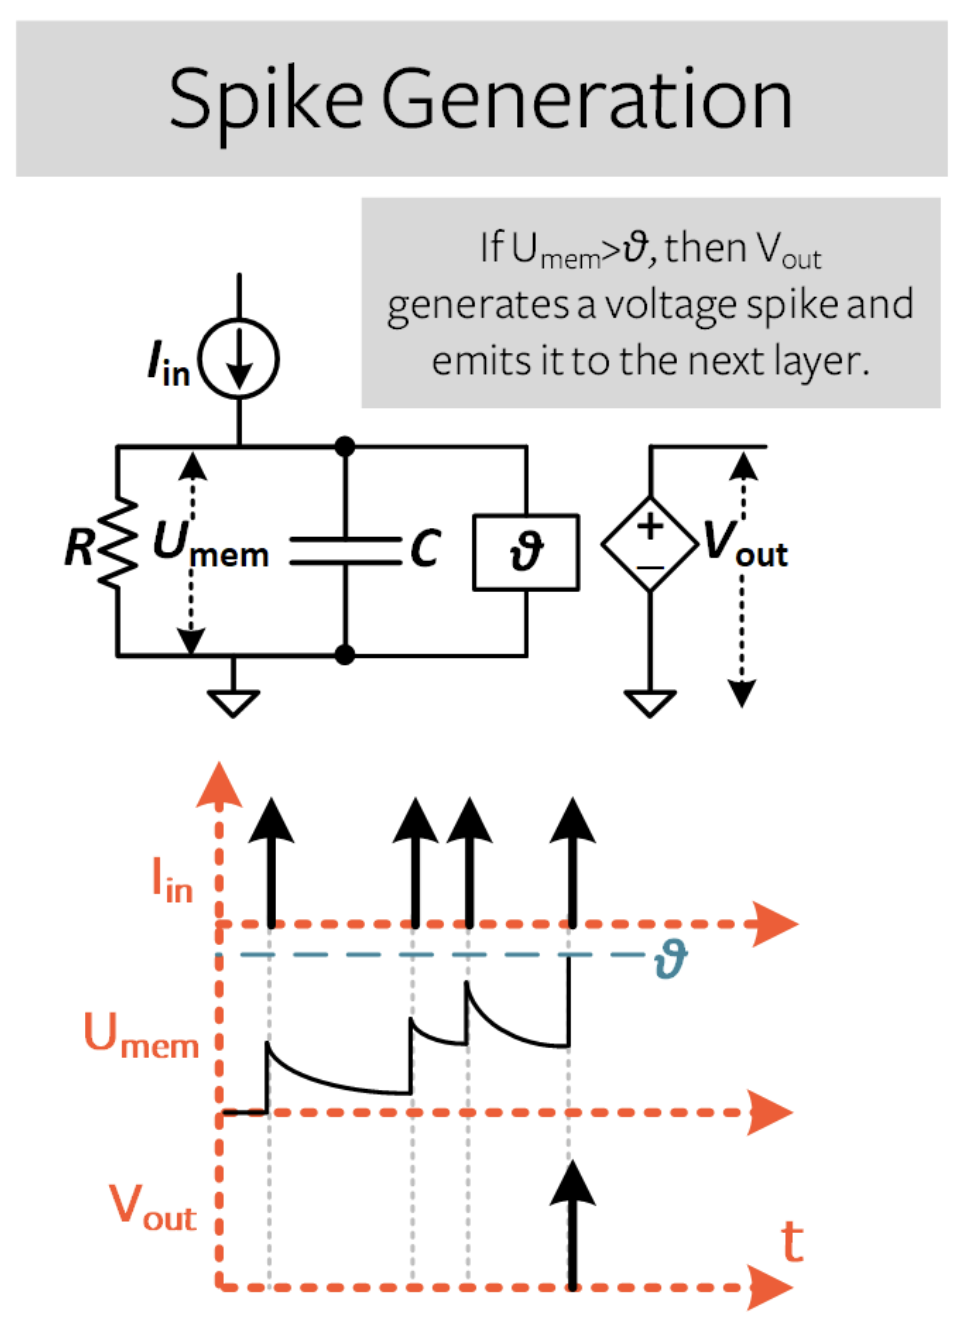
\includegraphics[width=\linewidth,trim=0 585bp 0 0,clip]{2_Background/background_figures/neuromorphic/LIF_diagram_2.png}
    \end{minipage}
    \hspace{0.1em}
    \begin{minipage}[b]{0.48\textwidth}
        \vspace{0pt}
        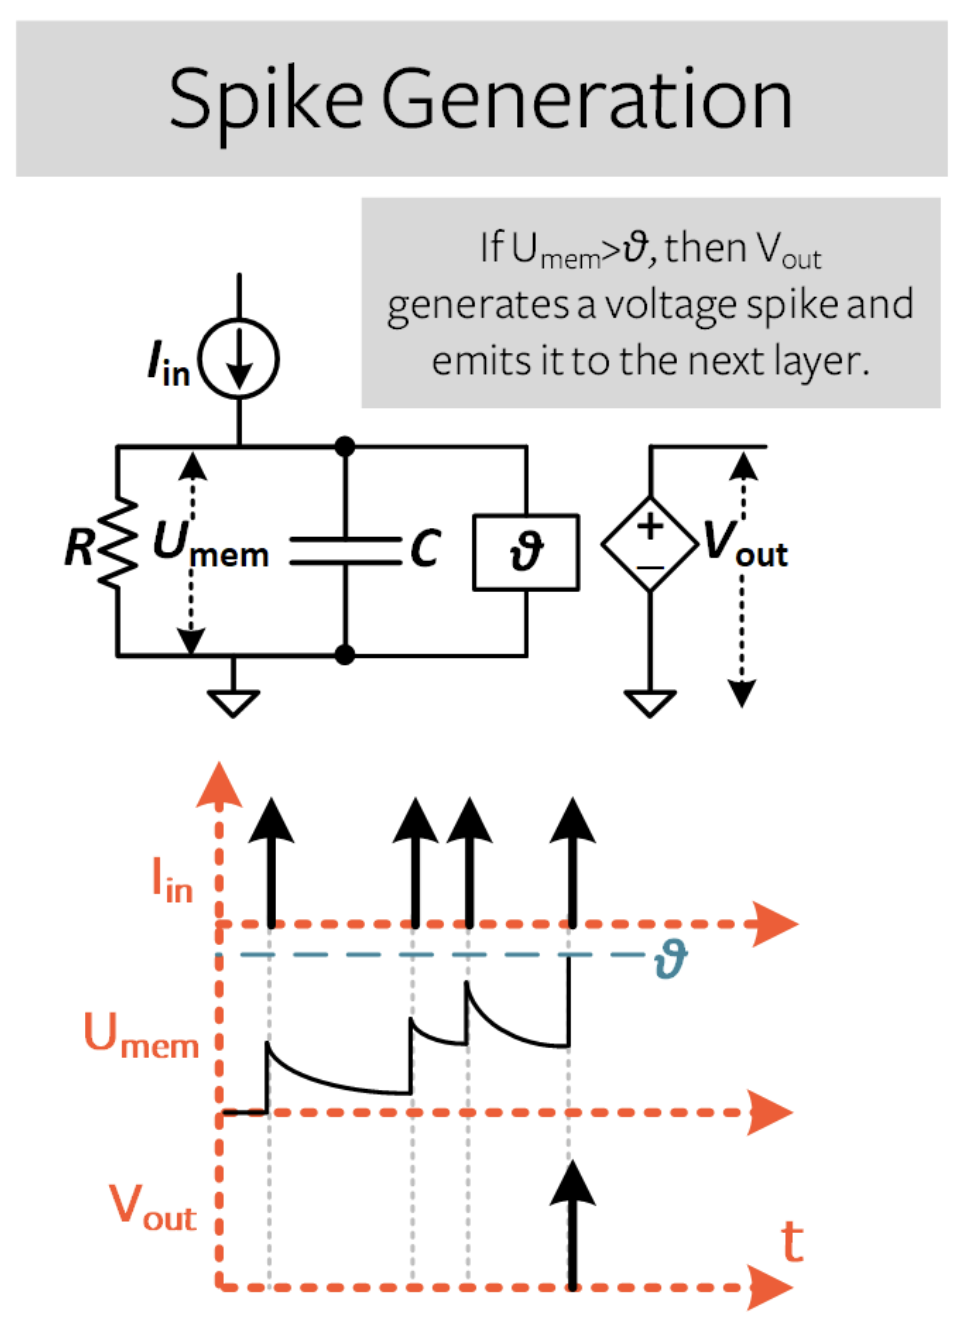
\includegraphics[width=\linewidth,trim=0 0 0 746bp,clip]{2_Background/background_figures/neuromorphic/LIF_diagram_2.png}
    \end{minipage}
    \caption{RC-circuit interpretation of a LIF neuron. Left: incoming current charges the membrane capacitor, while the resistor introduces leakage. Right: threshold crossing emits an output spike. The computational model abstracts the spike itself as a discrete event \cite{Eshraghian2023TRAININGLEARNING}.}
    \label{fig:lif_circuit}
\end{figure}

In continuous time,
\begin{equation}
    \tau_m \frac{\mathrm{d}V(t)}{\mathrm{d}t}
    =
    -\left(V(t)-V_{\mathrm{rest}}\right) + RI(t),
    \label{eq:lif_continuous_background}
\end{equation}
where $\tau_m=RC$ is the membrane time constant. Setting the resting potential to zero and discretising the dynamics gives the form used later in the report,
\begin{equation}
    V[t+1]
    =
    \underbrace{\beta V[t]}_{\text{decay}}
    +
    \underbrace{WX[t+1]}_{\text{weighted input}}
    -
    \underbrace{S[t]V_{\mathrm{thr}}}_{\text{reset}},
    \qquad
    \beta = e^{-\Delta t/\tau_m},
    \label{eq:lif_background_redraft}
\end{equation}
\begin{equation}
    S[t]
    =
    \begin{cases}
        1, & \text{if } V[t] > V_{\mathrm{thr}}, \\
        0, & \text{otherwise}.
    \end{cases}
    \label{eq:lif_spike_background}
\end{equation}
Here $X[t]$ is the input spike vector, $W$ contains synaptic weights, $\beta$ is the decay factor, and $S[t]$ is the emitted spike. Equation~\ref{eq:lif_background_redraft} uses a subtractive reset: after firing, the threshold is removed from the membrane voltage rather than forcing the voltage immediately to zero. This is the basic circuit element used throughout the report.

The engineering motivation for computing with spikes can be summarised by three properties: spikes, sparsity, and static suppression \cite{Eshraghian2023TRAININGLEARNING}. First, a spike is treated as a discrete event rather than a high-precision activation value. Second, neurons are often inactive, so sparse representations can reduce unnecessary memory access and arithmetic. Third, event-driven processing suppresses updates when no new information arrives. Neuromorphic hardware can exploit these properties using asynchronous communication between spiking neurons; large digital systems such as TrueNorth demonstrated million-neuron event-driven processors \cite{Merolla2014AInterface}. These properties do not automatically make every SNN efficient, but they motivate models that could later be mapped to neuromorphic hardware.

Modern trainable SNNs often use surrogate gradients. The spike function is non-differentiable, so during backpropagation its derivative is replaced with a smooth approximation. Forward simulation still uses spikes, while the backward pass uses a differentiable surrogate. This allows SNNs to be trained using deep-learning tools while retaining spiking dynamics \cite{Eshraghian2023TRAININGLEARNING}. In this project, the final trainable model uses SNN readouts to test whether the biologically structured pathway features are more useful than raw waveform or cochlear-raster inputs.

\section{Coincidence Detection, Population Codes, and Biological Baselines}
\label{sec:coincidence_background}

The threshold operation makes an LIF neuron useful for coincidence detection, displaying similar behaviour to logic gates. Neurons as logic gates was part of the original abstraction of artificial neurons proposed by McCulloch and Pitts \cite{Mcculloch1990AN}. Consider two excitatory inputs with positive weights, with weights representing synaptic strength (where synapses are the connections between neurons). If the firing threshold is lower than either weight, either input can trigger a spike and the neuron behaves approximately like an OR gate. If the threshold is higher than either individual weight but lower than their sum, both inputs must arrive within the membrane integration window and the neuron behaves like a time-sensitive AND gate. The same idea generalises to a $k$-of-$n$ criterion by setting the threshold relative to the summed input weights. The gate analogy is not exact: membrane leakage, refractory behaviour, and spike timing give the neuron dynamics that a Boolean gate does not have. Temporal coincidence selectivity depends strongly on the membrane time constant $\tau_m$, or equivalently the decay factor $\beta$ in Equation~\ref{eq:lif_background_redraft}. Slower decay broadens the integration window and allows more widely separated inputs to sum, while faster decay imposes a stricter coincidence criterion. Figure~\ref{fig:coincidence_detection_background}B illustrates this spatial and temporal integration.

This time-sensitive threshold operation is central to the distance and azimuth pathways. The classical Jeffress model was proposed for binaural sound localisation \cite{Jeffress1948ALocalization}. Signals from the left and right ears travel through delay lines of different lengths. For a given ITD, one pair of delayed signals arrives simultaneously at a coincidence detector, producing its strongest response. Different coincidence neurons therefore correspond to different candidate ITDs and, over the frontal field, different candidate azimuths. Figure~\ref{fig:coincidence_detection_background}A illustrates this place-code interpretation.

\begin{figure}[H]
    \centering
    \begin{minipage}[c]{0.33\textwidth}
        \centering
        \textbf{\large A}\\[0.5ex]
        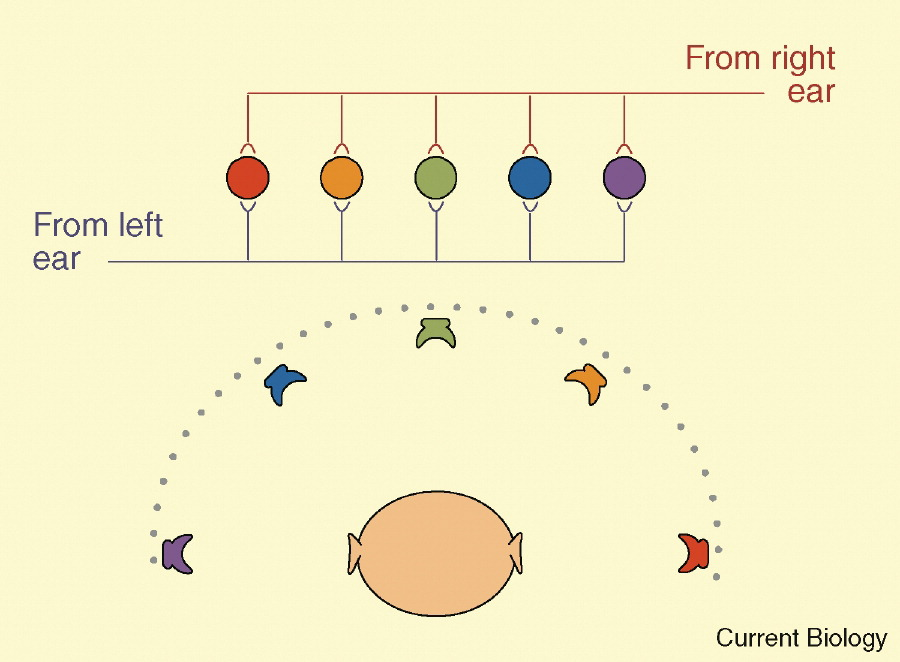
\includegraphics[width=\linewidth]{2_Background/background_figures/coincidence/Jeffress.jpg}
    \end{minipage}
    \hfill
    \begin{minipage}[c]{0.64\textwidth}
        \centering
        \textbf{\large B}\\[0.5ex]
        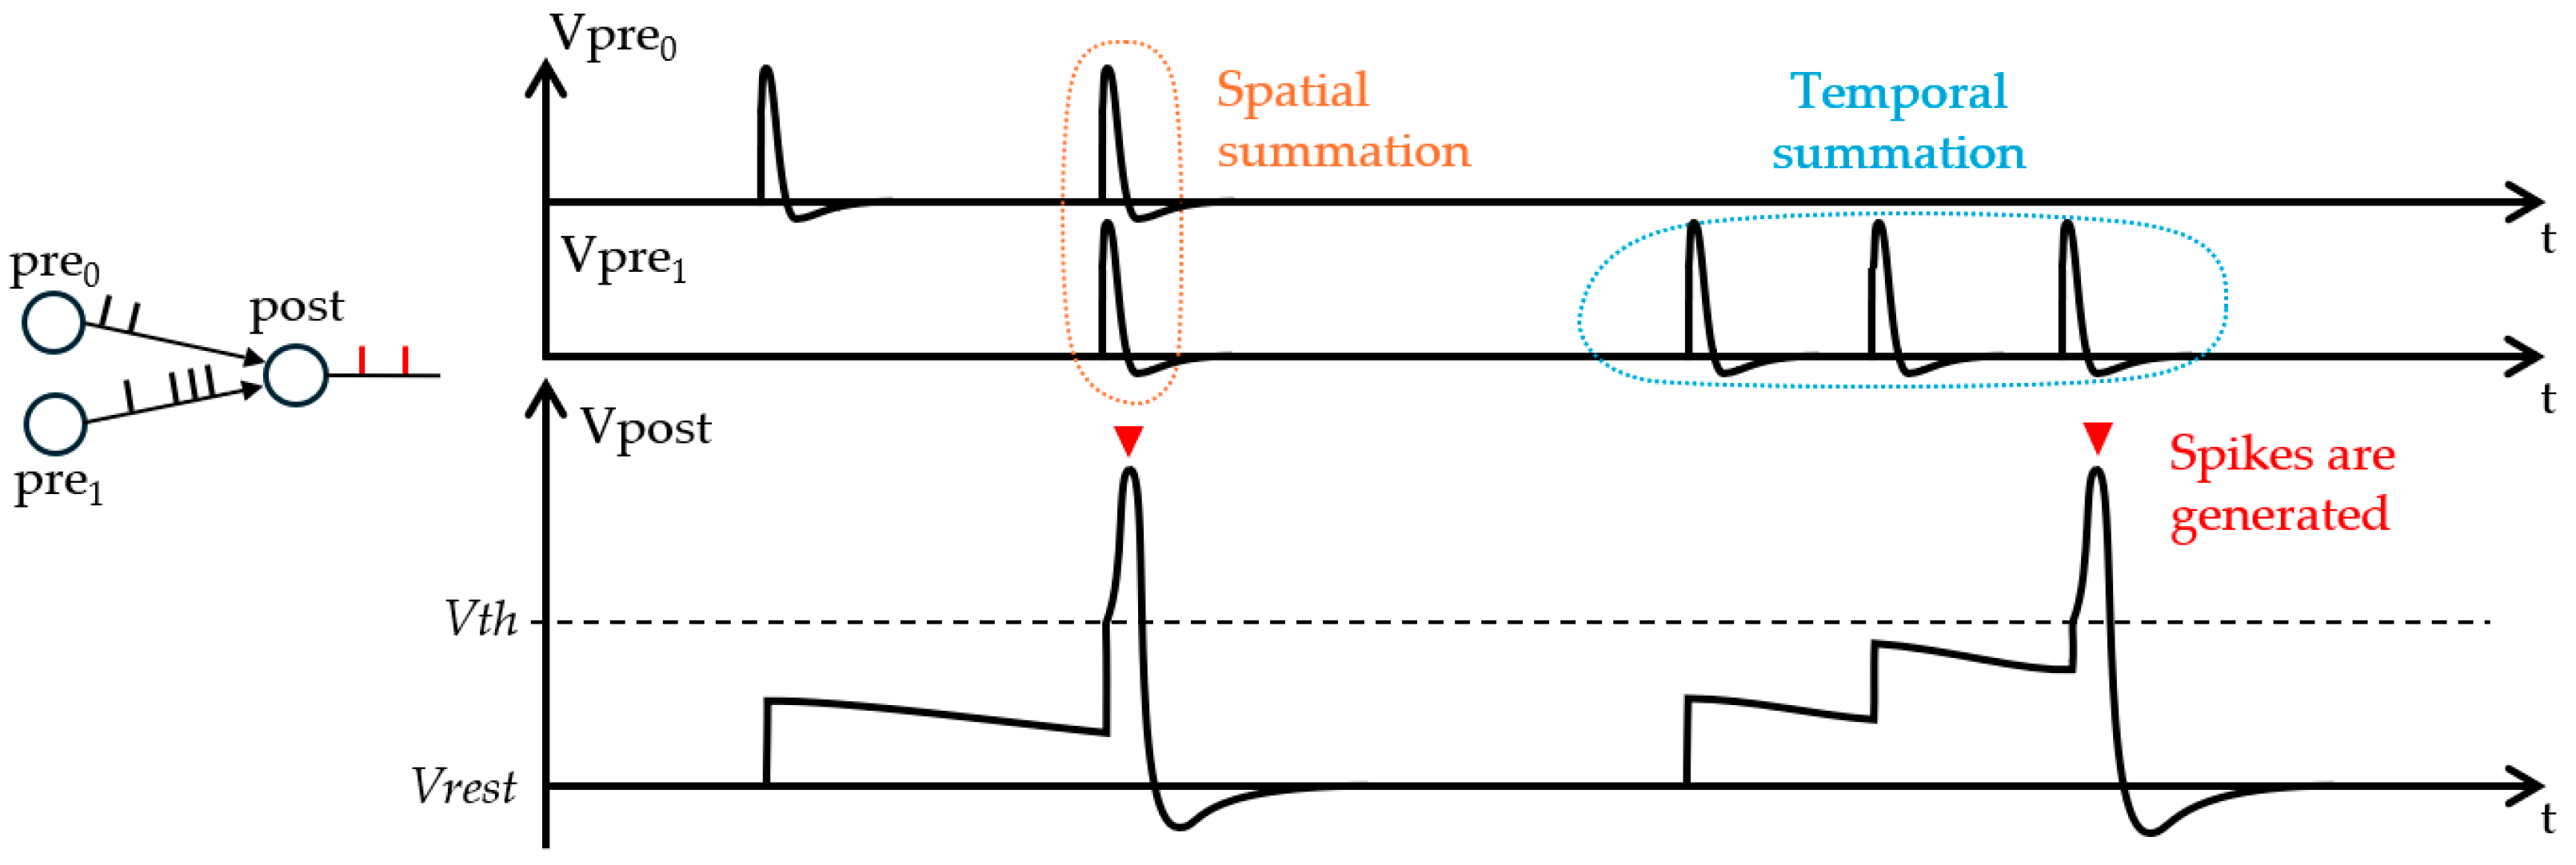
\includegraphics[width=\linewidth]{2_Background/background_figures/coincidence/coincidence.png}
    \end{minipage}
    \caption{A: Jeffress-style binaural delay-line model. Different internal delays align the left- and right-ear signals for different directions of arrival, causing the corresponding coincidence detector to respond most strongly \cite{Mosadeghzad2015SaliencyHumanoids}. B: spike generation in a post-synaptic neuron through spatial and temporal integration of pre-synaptic spikes. Membrane leakage returns the potential towards its resting value, and a spike is emitted when the integrated potential reaches the threshold \cite{Danneville2024ASystems}.}
    \label{fig:coincidence_detection_background}
\end{figure}

The distance pathway adapts the same computational idea to an active call-echo comparison. Instead of comparing left and right ear signals, it compares the returning echo with an internal corollary discharge reference for the emitted call. A bank (or set) of candidate internal delays shifts one signal relative to the other. The coincidence neuron whose delay best compensates for the echo ToF receives the most closely aligned inputs. This maps time delay into a population of candidate distances. The biological analogue is a population of FM-FM delay-tuned neurons, which respond selectively to combinations of emitted-call and echo components separated by particular delays \cite{Suga2015NeuralBat,Suzuki2017AcuityBats}. These neurons have been found anatomically in the auditory cortex of bats \cite{Suga1979NeuralBat}.

\subsection{Population Codes and Hyperacuity}

A nearest-neuron readout would limit resolution to the spacing between delay-tuned channels. Bat behaviour indicates that the actual readout is more precise. FM bats have been reported to discriminate echo-delay differences below 60~$\mu$s, corresponding to approximately 1~cm of range under a simple round-trip calculation \cite{Simmons1973TheBats}. Reviews also discuss sub-millimetre performance in specialised jitter experiments \cite{Ulanovsky2008WhatBrain}. Indicative angular scales are similarly small: approximately $1$-$2^\circ$ for azimuth and approximately $3^\circ$ for elevation are useful order-of-magnitude comparators \cite{Ulanovsky2008WhatBrain,Lawrence1982EcholocationTargets}. These behavioural tasks are not directly equivalent to the model evaluation in this report, but they motivate a readout that can estimate values between discrete neural tuning centres.

This sub-resolution precision is often described as hyperacuity. Population decoding provides a plausible explanation: information is read from the pattern of responses across many neurons rather than from the identity of the single most active neuron. Suzuki and Suga model this idea for delay-tuned neurons using the centre location of the distributed response \cite{Suzuki2017AcuityBats}. The exact biological mechanism remains debated, but the engineering consequence is clear. A smooth population response can be decoded between the centres of neighbouring neurons.

\begin{figure}[H]
    \centering
    \begin{minipage}[t]{0.48\textwidth}
        \vspace{0pt}
        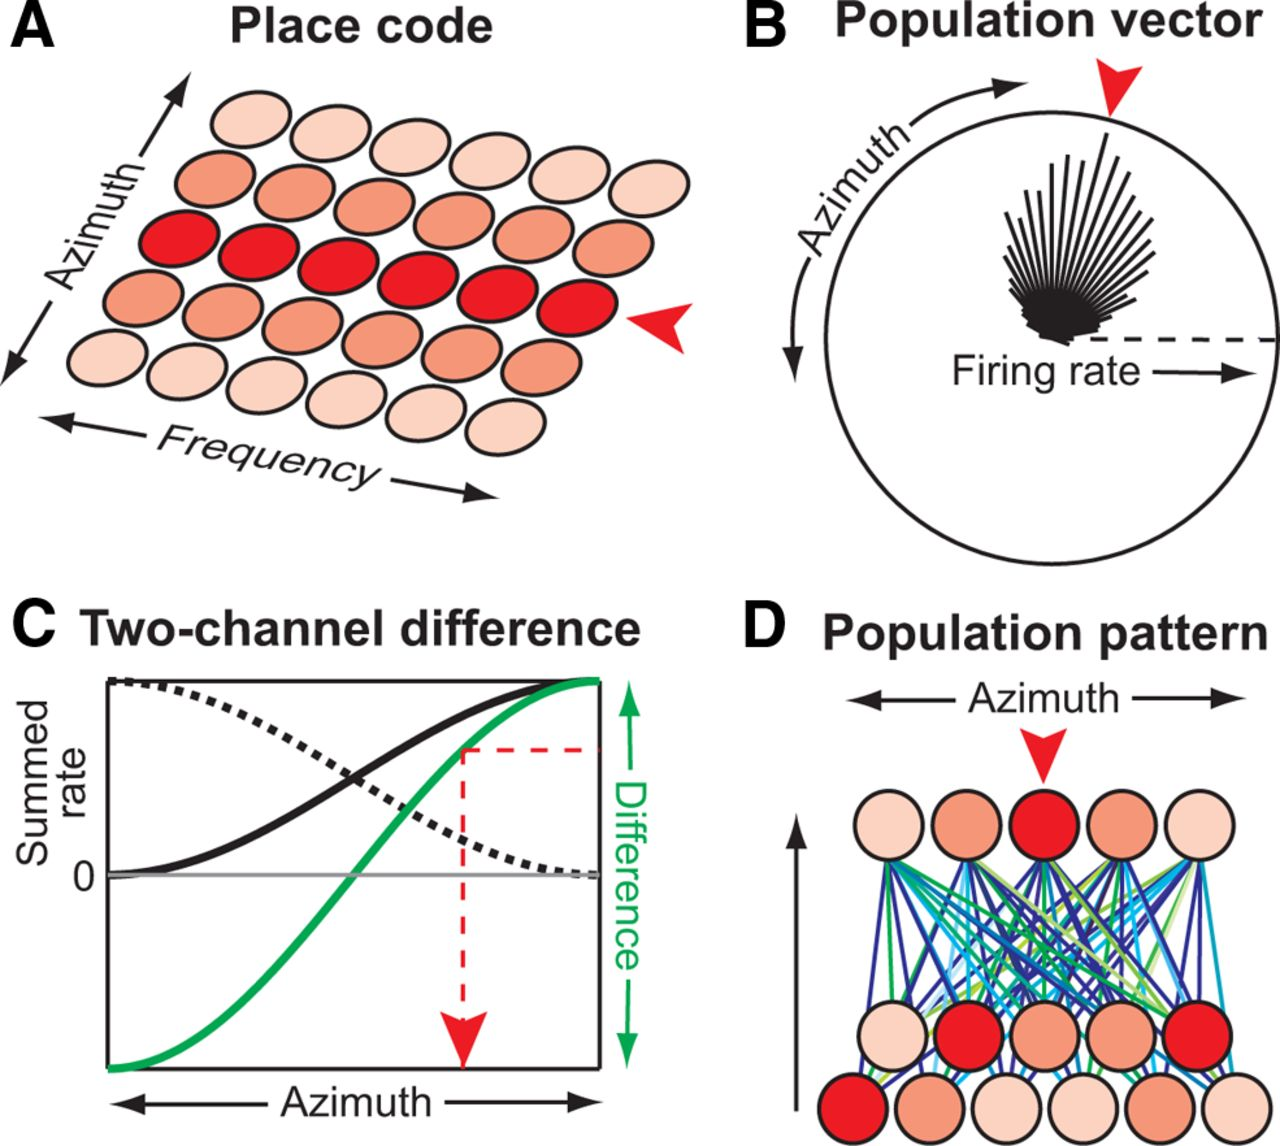
\includegraphics[width=\linewidth,trim=0 137.5bp 0 0,clip]{2_Background/background_figures/coincidence/population.jpg}
    \end{minipage}
    \hfill
    \begin{minipage}[t]{0.48\textwidth}
        \vspace{0pt}
        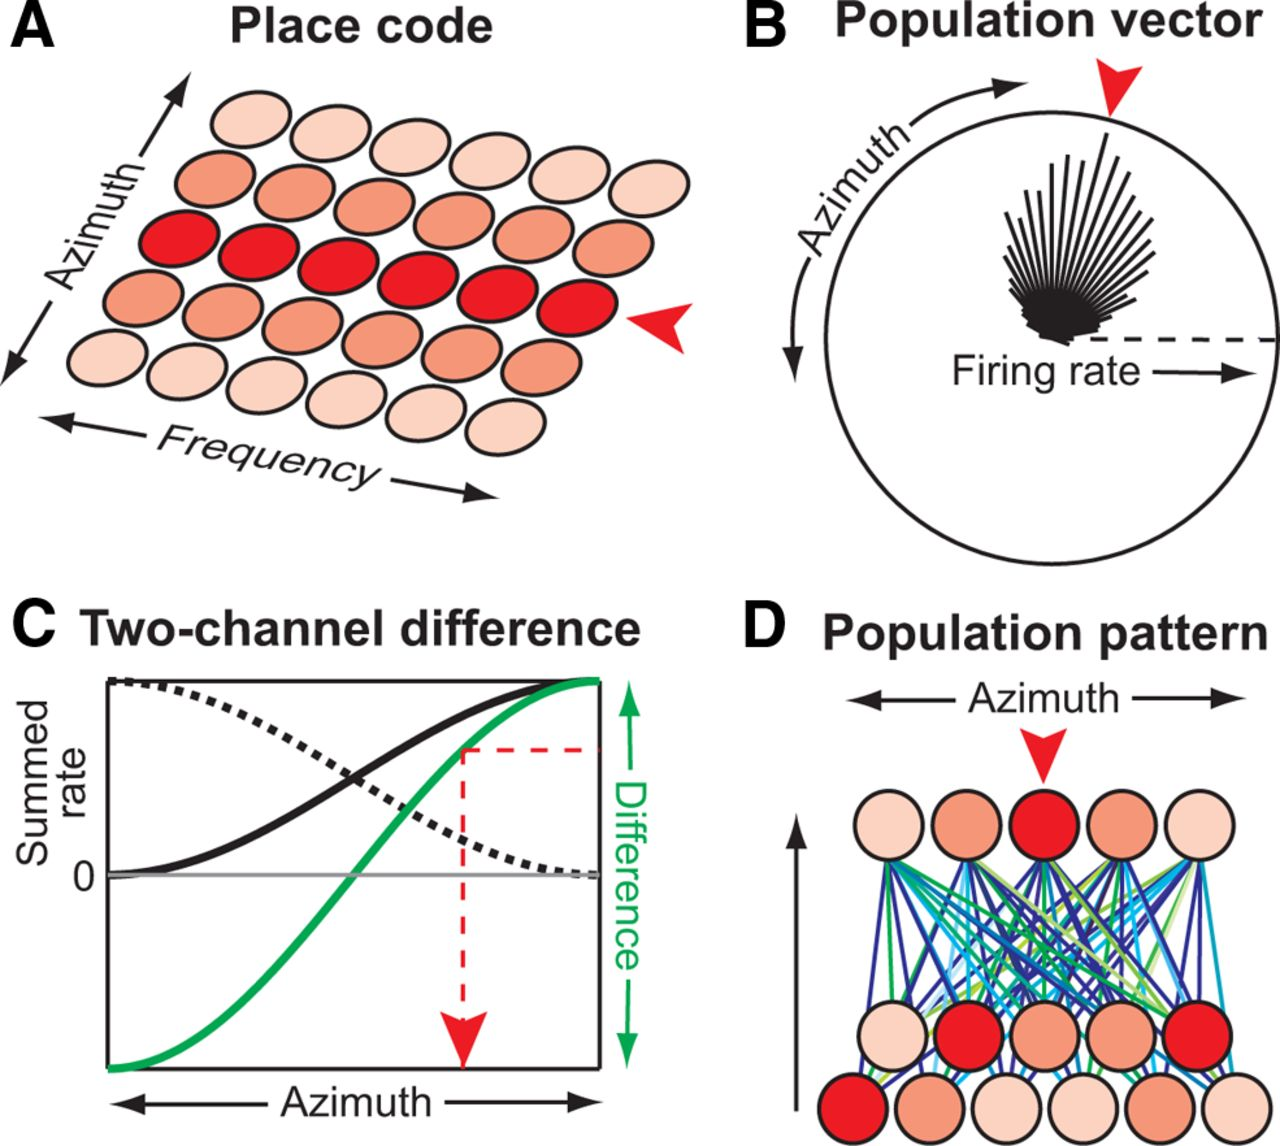
\includegraphics[width=\linewidth,trim=0 0 0 137.5bp,clip]{2_Background/background_figures/coincidence/population.jpg}
    \end{minipage}
    \caption{Examples of neural population-decoding schemes for azimuth. A: place-code, B: population-vector, C: two-channel-difference and D: population-pattern readouts \cite{Day2013DecodingPatterns}.}
    \label{fig:population_decoding}
\end{figure}

Figure~\ref{fig:population_decoding} illustrates several ways in which a distributed response can be decoded. This motivates the centre-of-mass (COM) and continuous-attractor readouts evaluated later in the report. A continuous attractor neural network (CANN) is a recurrent population in which local excitation and broader inhibition can stabilise a bump of activity. CANNs are established models for representing continuous variables such as direction or spatial location \cite{ContinuousScholarpedia,Li2024DynamicsNetworks,Wu2016ContinuousRepresentation}. The detailed dynamics of these networks are outside the scope of this report. They should be understood here as candidate models for the ``encoding of simple continuous features in neural systems'' described by Wu et al.\ \cite{Wu2016ContinuousRepresentation}. In this report, the CANN is treated as one possible SC-style readout abstraction rather than as a proven model of bat hyperacuity. The upstream pathway produces a population response, and the recurrent readout can smooth or stabilise it before decoding.

Rate coding is the other relevant abstraction. A fully spiking population produces individual spike trains, but many downstream computations can use average spike count or firing rate over a short window. Rate is a summary of spiking activity rather than a replacement for it. In the model, explicit spike rasters are retained where timing matters, while rate-coded population vectors are used where the relevant information is the strength of activity across candidate coordinates.

\section{Current Models and Project Gap}

Biological sensing systems have long served as inspiration for engineered localisation systems. Echolocating bats are particularly relevant because they perform active acoustic sensing using compact biological hardware in complex environments. The potential engineering value of these strategies has motivated substantial work in biologically inspired radar and sonar \cite{Balleri2017Biologically-inspiredNature}. Existing models span conventional signal processing, probabilistic cue integration, artificial neural networks, and neuromorphic systems \cite{Li2003ALocalization,Willert2006ALocalization,Carlini2024AuditoryReview}. They can be organised into several complementary research directions.

\subsection{Learned End-to-End Localisation and Reconstruction}

Recent machine-learning systems show that spatial information can be inferred directly from binaural audio. Deep neural networks trained on large acoustic datasets can estimate sound-source location and reproduce aspects of human localisation behaviour \cite{Francl2022DeepEnvironments,Baby2021AApplications}. Related active-echolocation systems solve richer reconstruction tasks. BatVision uses emitted chirps and binaural echoes to predict scene depth maps and grayscale images, while Bat-G net reconstructs high-resolution three-dimensional target representations from ultrasonic echoes \cite{ChristensenBatVision:Ears,HwangBat-GEchoes}.

These systems demonstrate that learned models can exploit the spatial information contained in echoes. Bat-G net is a particularly relevant conceptual comparator because its encoder is organised around an abstraction of the bat central auditory pathway, as shown in Figure~\ref{fig:bat-G_net}. However, its internal representations are implemented primarily through learned convolutional operations rather than explicit spiking cue pathways. Such models prioritise reconstruction performance, whereas this project asks whether interpretable distance, azimuth, and elevation populations remain useful before the final trainable stage.

\begin{figure}[H]
    \centering
    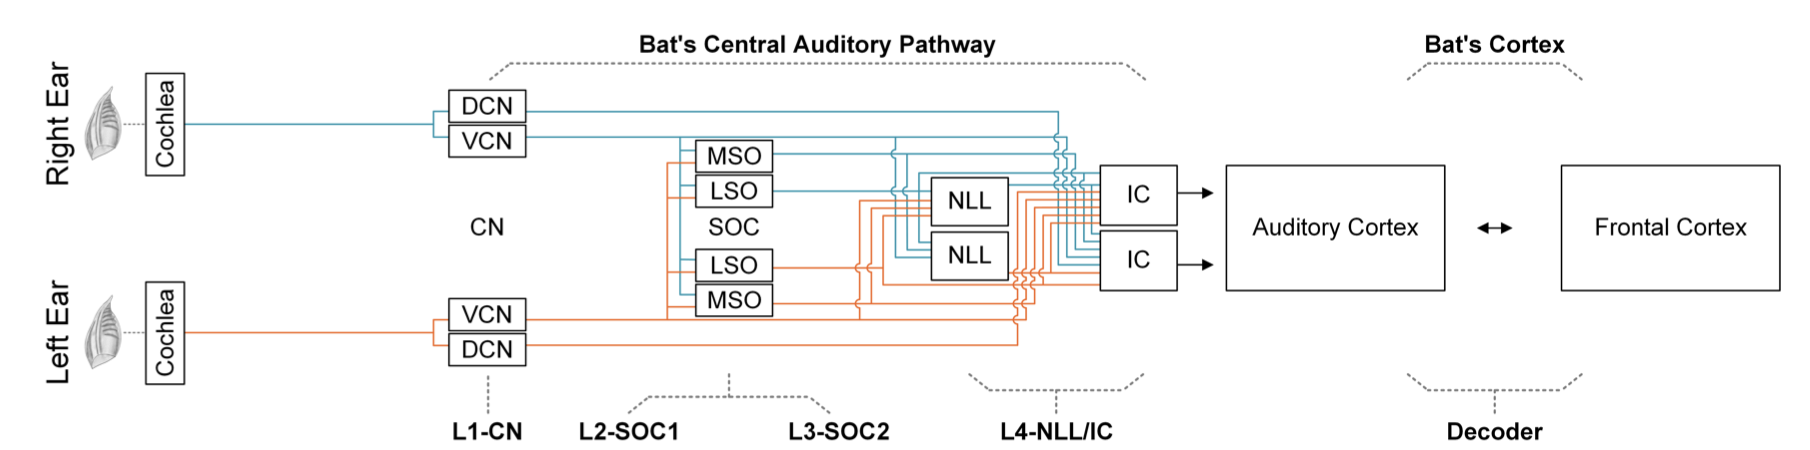
\includegraphics[width=\textwidth]{2_Background/background_figures/neuromorphic/bat-G_net.png}
    \caption{Simplified diagram of the anatomical connections of a bat's auditory system and the architecture of the proposed Bat-G network \cite{HwangBat-GEchoes}.}
    \label{fig:bat-G_net}
\end{figure}

\subsection{Biophysical and Functional Auditory Subsystem Models}

A second body of work models individual stages of auditory processing in greater biological detail. Cochlear models range from efficient filterbank approximations to detailed simulations of basilar-membrane mechanics, nonlinear transduction, and auditory-nerve responses \cite{deBoer1980AuditoryI,Sieroka2006SemirealisticCochlea,Pennington2023ACortex,ApplyingAudiology}. Neuromorphic cochlear front ends commonly decompose a waveform into frequency channels, apply nonlinear transduction or rectification, and encode the resulting activity as spikes. For example, the Heidelberg spiking datasets use a biologically motivated artificial cochlea to convert audio waveforms into temporally structured spike trains \cite{Cramer2022TheNetworks}.

Beyond the cochlea, numerous models isolate particular localisation computations. These include ITD processing through delay lines and coincidence detection, ILD processing through opponent neural populations, and spectral-cue processing for elevation estimation \cite{Lazar2008FaithfulNeurons,Moro2022NeuromorphicTransducers,Tanveer2021EstimateStudy,OssesVecchiAProcessing}. Spiking implementations of auditory mechanisms have also been proposed, often drawing on pathways studied in birds or mammals \cite{Wall2012SpikingDifference,Goldsworthy2022ComputationalStimulation,Biswas2022ModelingOscillators}. This work provides useful mechanistic insight, but the models often address an individual component or a restricted localisation subproblem rather than a complete active three-dimensional echolocation pipeline.

The modular approach used in this report is designed to sit above this level of detail. Each simplified pathway can be inspected independently and could later be replaced with a more biophysically detailed subsystem where that additional complexity is justified.

\subsection{Neuromorphic Sound Localisation}

Neuromorphic sound-source localisation has received increasing attention, particularly for binaural azimuth estimation from ITD and ILD cues. Reviews identify a range of spiking and event-based systems motivated by MSO/LSO-style auditory-brainstem processing \cite{Danneville2024ASystems}. Some use engineered auditory front ends followed by trainable networks, while others implement specific neural mechanisms more directly.

The COMOB sound-localisation project is one of the closest methodological comparators to this work. It provides a public framework for training spiking neural networks to solve a binaural sound-localisation task using surrogate-gradient learning \cite{SpikingProject}. Its focus is passive sound-source localisation and ITD extraction rather than active pulse-echo object localisation. More generally, many neuromorphic systems prioritise task performance over an explicit, inspectable mapping between known acoustic cues and successive neural populations. This leaves room for models that retain interpretable cue-specific representations while still using trainable spiking networks where manual integration becomes difficult.

\subsection{Active Echolocation Simulation and the Remaining Gap}

A complementary research direction focuses on the acoustic environment experienced by an echolocating system. SonoTraceLab provides an open-source ray-tracing framework for simulating technical and biological sonar in complex scenes \cite{Jansen2024SonoTraceLabBats}. Studies of bat group echolocation and robotic sonar systems further illustrate the importance of realistic echoes, pinna effects, and environmental interference when evaluating active sensing \cite{Mazar2026Agent-basedEmergences,Schillebeeckx2011BiomimeticPinnae}.

Consequently, a gap remains between detailed subsystem models and learned end-to-end localisation systems. The former offer mechanistic insight but are rarely integrated into complete object-localisation architectures. The latter can achieve impressive localisation or reconstruction performance but often replaces explicit auditory computations with learned internal representations. Based on the research conducted, few systems combine active three-dimensional echolocation, explicit cue-specific auditory pathway abstractions, intermediate spike representations, interpretable population codes, and a trainable spiking fusion stage within one modular localisation pipeline.

The model developed in this report occupies this intermediate position. It does not attempt a detailed anatomical simulation of the bat auditory system. Instead, it implements the principal computations associated with distance, azimuth, and elevation estimation using simplified pathway abstractions. These pathways expose intermediate representations linked to specific acoustic cues. A small trainable SNN is then used for feature fusion and residual correction. This design aims to preserve the interpretability and modularity of biologically inspired processing while retaining the flexibility of learned neural models.
